%! TeX root: thesis.tex
\section{Framework}
In diesem Abschnitt soll es um das Implementierte Framework gehen.
Aus den theoretischen Grundlagen lässt sich schließen, dass 
folgende Daten (-Strukturen) unbedingt im Framework implementiert sein sollten:

\begin{enumerate} \label{tac}
  \item Drei Address Code Instruktionen:\\ 
    Um einzelne Instruktionen zu modellieren zu können brauchen diese einen
    eigenen Datentyp, um Eigenschaften wie Sprünge, konstante Werte oder
    gelesene und geschriebene Variablen darstellen zu können.
  \item Drei Address Code Operationen:\\
    Da es 16 verschiedene Operationen gibt, von denen sich auch noch einige
    gruppieren lassen, ist es sinnvoll, ein Enum zu schreiben, um mit 
    switch-Statements arbeiten zu können.
  \item Grundblöcke:\\ 
    Die Grundblockklasse soll speichern, wo im 3-Address-Code Programm
    einzelne Grundblöcke anfangen, aufhören und zu welchen Addressen sie springen.
  \item Drei Address Code: \\ 
    Diese Klasse soll das gesamte Programm modellieren, also alle Instruktionen
    speichern und die Grundblöcke generieren.
\end{enumerate}
Daraus ergibt sich folgendes Klassendiagramm(\cref{fig:3AC-classes}):
\begin{figure}[h]
  \centering
  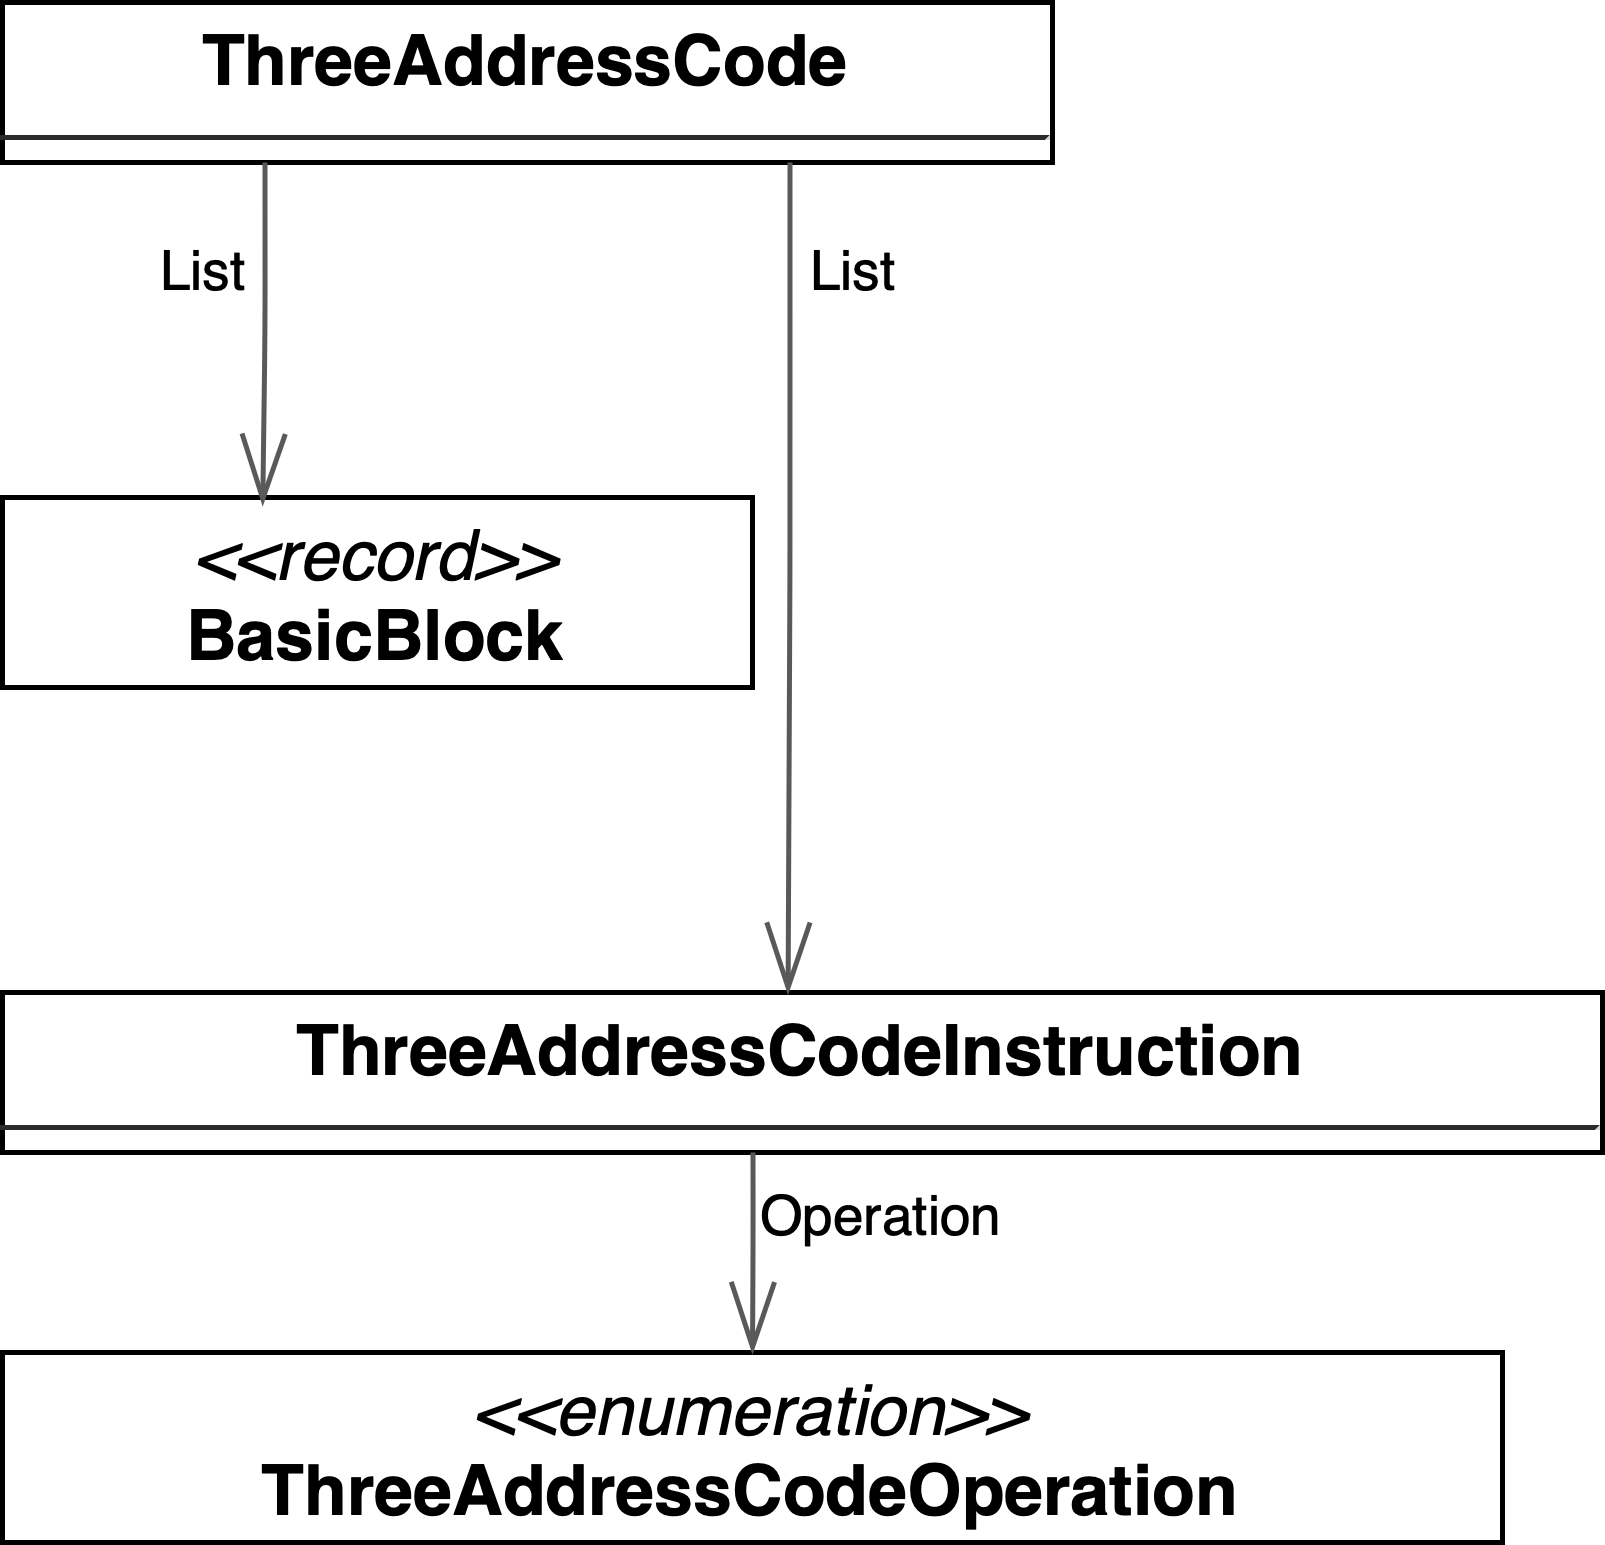
\includegraphics[width=0.5\textwidth]{fig/3AC_classes.png}
  \caption{Die Drei Address Code Klassen im Überblick}%
  \label{fig:3AC-classes}
\end{figure}


\newpage
Da der Usecase dieses Frameworkes das Visualisieren von Algorithmen ist, 
braucht es folglich eine Möglichkeit, den 3-Address-Code zu visualisieren.
Hier wurde sich für eine Tabelle entschieden, da eine Instruktion in acht Zellen
\footnote{$if\ Y\ relOp\ X\ goto\ L$ ist mit 6 Elementen die längste legale 3-Address-Code Instruktion,
dazu wird noch eine Zelle für die aktuelle Instruktion und eine für Kommentare hinzugefügt} 
aufgeteilt werden kann. Da es sich bei einem Programm immer um
eine Liste von Instruktionen handelt, ergibt sich so ein Zweidimensionales Feld an Daten.
Außerdem sollen auch die Daten die wir aus unseren Analysen erheben
angezeigt werden. Auch hier ist eine Tabelle sinnvoll.\\

Um Kontrollflussgraphen anzeigen zu können, soll es ausserdem möglich sein
Graphen anzuzeigen.\\

Mit einer Toolbar soll es möglich sein mit dem aktuell geladenen Plugin zu interagieren.\\


Aus diesen Anforderungen ergibt sich folgendes Klassendiagramm(\cref{fig:gui-classes}):\\
\begin{figure}[h]
  \centering
  \vspace{-15pt}
  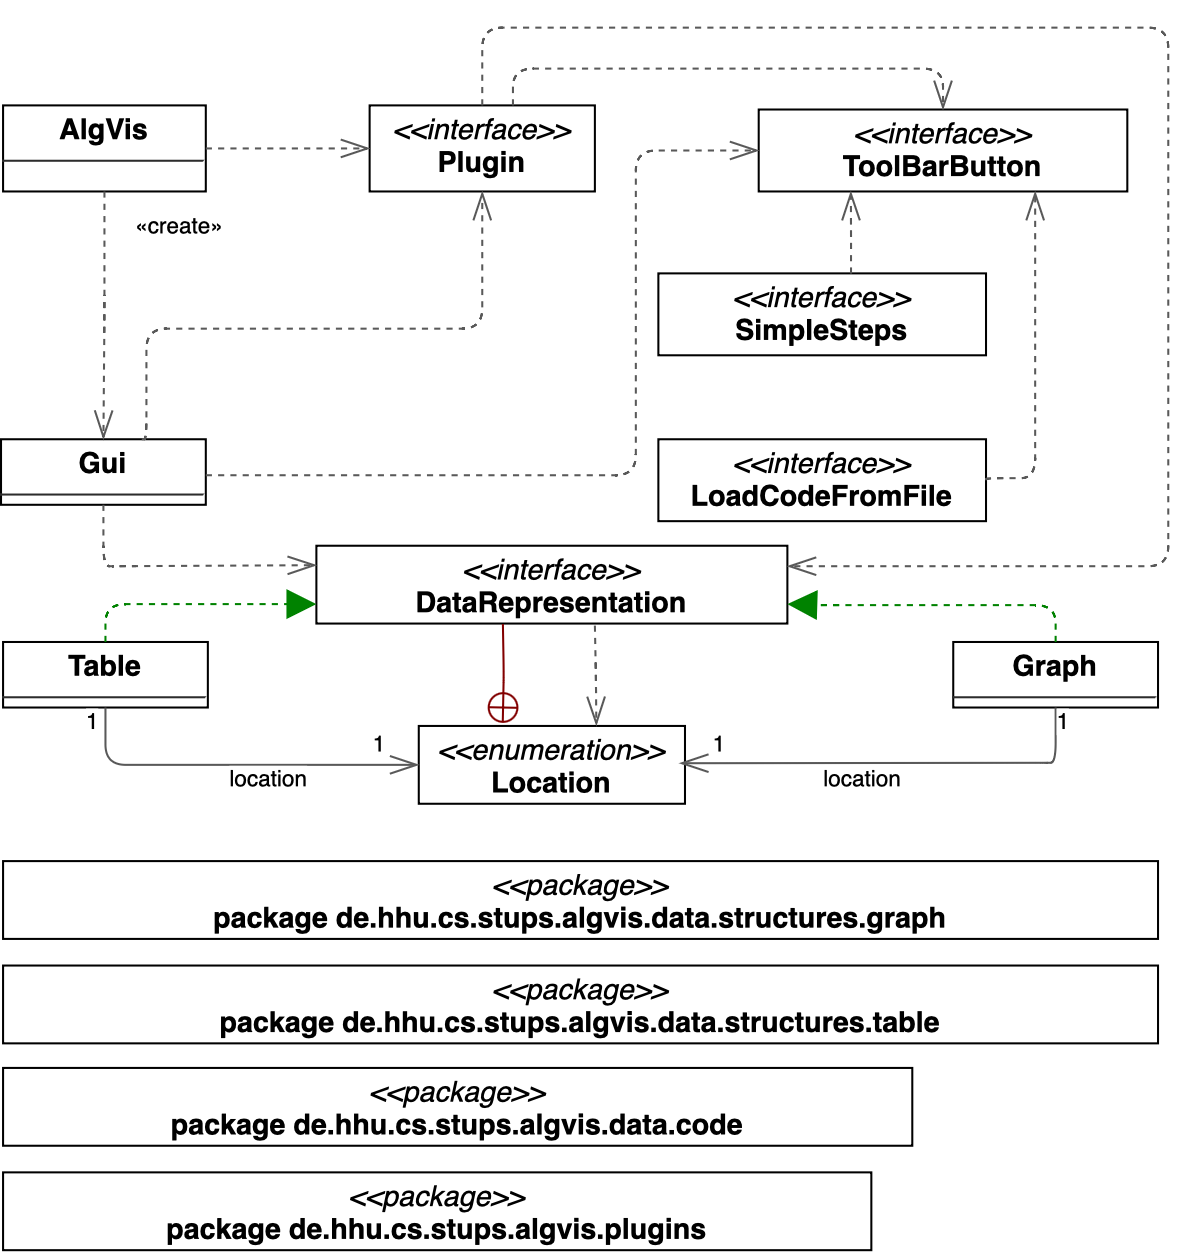
\includegraphics[width=0.75\textwidth]{fig/GUI_classes.png}
  \vspace{-10pt}
  \caption{Klassenstruktur der GUI-Klassen}%
  \label{fig:gui-classes}
\end{figure}
\vspace{-20pt}

\newpage
\begin{itemize}
  \item Die Klasse \textit{AlgVis} gilt hier (\cref{fig:gui-classes}) als Entrypoint. 
    Sie lädt alle Plugins, erstellt ein \textit{Gui} Objekt und übergibt diesem die Plugins.
  \item Das Interface \textit{Plugin} definiert welche Methoden neue Plugins
    beziehungsweise Algorithmen
    benötigen um hinzugefügt zu werden, diese werden in\\
    \textit{de.hhu.cs.stups.algvis.plugins} implementiert.
  \item Zudem definiert das Interface \textit{ToolBarButton} wie Buttons der ToolBar,
    welche im nächsten Kapitel im Detail erklärt wird, implementiert werden können.
    Beispiele dafür liefern das \textit{SimpleSteps} und \textit{loadCodeFromFile} Plugin,
    welche vordefinierte Buttons anbieten.
  \item Die Packages endend auf \textit{graph} und \textit{table} enthalten hierbei Helferklassen 
    für die jeweiligen Komponenten, hierzu später mehr.
  \item Im Package \textit{de.hhu.cs.stups.algvis.data.code} sind die vorhin genannten Datenstrukturen
    für 3-Address-Code, Grundblöcke, 3-Address-Code-Instruktionen\\ 
    und -Operationen implementiert.
\end{itemize}

\subsection{Gui} 
Die \textit{Gui} Klasse ist das Herzstück der Visualisierung. Hier wird ein \textit{JFrame},
also ein GUI Fenster der Java Standardlibrary \textit{Swing} geladen. In ihr befinden sich
drei GUI-Elemente, auch aus der \textit{Swing}-Library:
\begin{enumerate}
  \item Eine Menüleiste, in der über ein Dropdown alle Plugins aufgerufen werden können.
  \item Ein \textit{JPanel}, welches im folgenden \textit{ContentPanel} genannt wird, 
    da sich in ihm alle grafischen Elemente des aktuell genutzten Plugins befinden.
    In ihm können Plugins Objekte die das Interface
    \textit{DataRepresentation} implementieren einfügen.
    Die Klassen \textit{Table} und \textit{Graph} implementieren dieses Interface bereits. 
    Sollte später ein Plugin eine andere Art der Darstellung benötigen,
    kann dieses das Interface mit einer anderen \textit{awt}-Komponente implementieren.
    Zum Start des Frameworks zeigt es einen SplashScreen (\cref{fig:screenshot_splashScreen}) mit dem Schriftzug \glqq welcome\grqq an.
  \item Und eine \textit{JToolBar}.\\
    Da die meißten Plugins ähnliche Funktionalitäten haben, wie zum Beispiel
    das schrittweise Durchlaufen eines Algorithmus, 
    wurde ein GUI-Element hinzugefügt in dem Buttons zur Kontrolle des Plugins
    hinzugefügt werden können. Diese ist auf der Abbildung(\cref{fig:screenshot_splashScreen})
    nicht zu sehen, da aktuell kein Plugin geladen ist und somit auch kein Buttons angezeigt werden
\end{enumerate}


\newpage
\begin{figure}[h!]
  \centering
  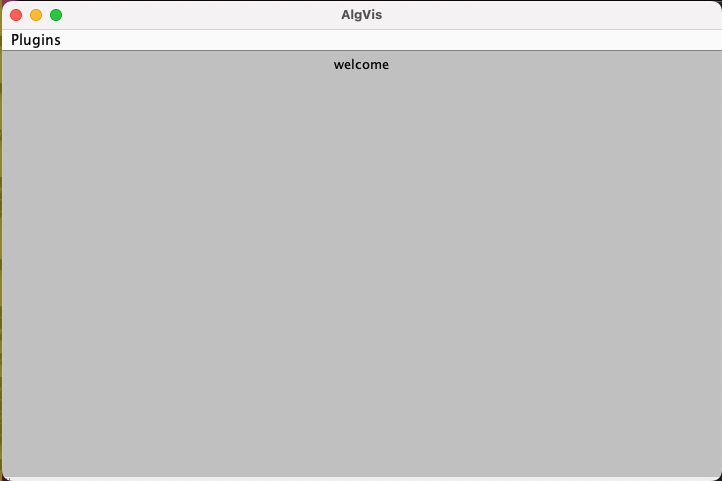
\includegraphics[width=0.7\textwidth]{fig/Screenshot_SplashScreen.png}
  \caption{Ansicht des Programmes direkt nach Start}
  \label{fig:screenshot_splashScreen}
\end{figure}



\subsection{Darstellen von Daten}
\begin{wrapfigure}[14]{r}{0.3\textwidth}
  \vspace{-15pt}
  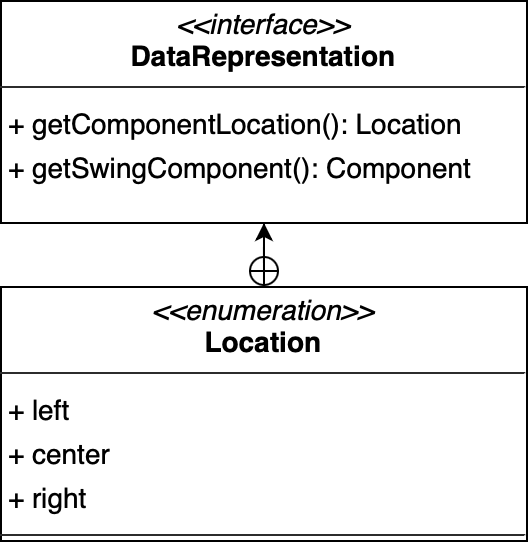
\includegraphics[width=0.3\textwidth,]{fig/GUI_DataRepresentation.png}
  \vspace{-15pt}
  \caption{Das DataRepresentation Interface und sein Location enum}
  \label{fig:DataRepresentation}
  \vspace{-30pt}
\end{wrapfigure}
Um grafische Elemente im \textit{ContentPanel} darzustellen wird das Interface \textit{DataRepresentation}
von Gui-Klassen implementert. Dadurch kann auf zwei Methoden zugegriffen werden:
\begin{itemize}
  \item \textit{getSwingComponent()} gibt die \textit{awt}-Komponente zurück, welche dem \textit{ContentPanel}
    hinzugefügt wird.
\item Durch die Methode \textit{getComponentLocation()} wird bestimmt an welcher
  Position im \textit{ContentPanel} diese angezeigt wird. Dies wird 
\end{itemize}




Das Enum \textit{Location} entscheidet hierbei wo im \textit{ContentPanel} das Gui-Objekt
angezeigt wird.\\

Für diese Arbeit wurden folgende Gui-Klassen implementiert:


\newpage
\subsubsection{Graphen}
\begin{wrapfigure}{r}{0.17\textwidth}
  \vspace{-10pt}
  \centering
  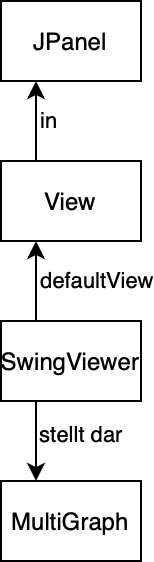
\includegraphics[width=0.1375\textwidth]{fig/GUI_Graph_rendering_pipeline.png}
  \caption{Rendering Pipeline eines Graphen}%
  \label{fig:graph-rendering-pipeline}
  \vspace{-10pt}
\end{wrapfigure}
Graphen werden durch die Klasse \textit{Graph} und zwei Subklassen 
\textit{Edge} und \textit{Node} realisiert(siehe \cref{fig:graph-classes}).
Da das Schreiben einer eigenen Engine für die Darstellung von Graphen
diese Bachelorarbeit übertreffen würde wurde entschieden eine externe Library
zu verwenden. Hier wurde sich für GraphStream\cite{GS}
entschieden.\\

Graphstream ist eine Library zum modellieren, analysieren und visualisieren von Graphen,
im Framework wird sie jedoch nur benutzt um Graphen zu visualisieren.\\
Um einen Graphen im \textit{ContentPanel} anzeigen zu lassen gibt 
die Methode \textit{getSwingComponent()} ein JPanel wieder,
in diesem JPanel befindet sich ein GraphStream \textit{View} Objekt welches von einem
\textit{SwingViewer} erstellt wird, welcher in einem eigenen Thread(siehe \cref{cde:graph-constructor}) einen
\textit{MultiGraph} rendert(siehe \cref{fig:graph-rendering-pipeline}).
Dies stellt die default Renderingstrategie dar\cite{GS_render}.\\
Graphstream bietet einige verschiedene Implementierungen von Graphen an, 
die je nach Usecase unterschiedliche Vorteile haben. Hier wurde sich dafür
entschieden nur die \textit{MultiGraph} implementierung zu verwenden, da es
möglich sein muss mehrere Kanten zwischen denselben zwei Knoten zu haben.
\footnote{Es wird die Möglichkeit benötigt eine Kante a>b und eine Kante b>a gleichzeitig darzustellen}
Diese Implementierung wird laut Dokumentation nur von einem \textit{MultiGraph}
implementiert.\cite{GS_graphs}\\

Nun wird im GUI ein leerer Graph angezeigt.\\
Um dem \textit{MultiGraph} nun einen Knoten hinzuzufügen benutzen wir 
die Methode \textit{addNode(String)}. Diese erwartet einen String als ID,
dementsprechen müssen alle Knoten die wir hinzufügen einen eindeutigen
String haben.\\
Um eine Kante hinzuzufügen wird die Methode \textit{addEdge(String, String, String, boolean)}
hierbei soll der erste String die eindeutige ID der Kante sein und die beiden folgenden Strings
die IDs der jeweiligen Aus- und Eingangsknoten.
Der Boolean-Wert gibt hierbei an ob die Kante eine gerichtete Kante ist, oder nicht.
Um Knoten oder Kanten zu entfernen gibt es die Methoden \textit{removeNode(String)}
und \textit{removeEdge(String)} die nach demselben Prinzip agieren.\\

Um das Aussehen eines Graphen anzupassen werden Attribute benutzt\cite{GS_data}.
Attribute können Graphen, Knoten und Kanten mit der Methode \textit{setAttribute(String, Object)}
hinzugefügt werden, hierbei ist der erste String das Attribut und das folgende
Objekt der Wert des Attributes. Im Falle dieser Arbeit sind zwei Attribute relevant:
\begin{itemize}
  \item Das gerenerelle \glqq look and feel\grqq des Graphen wird durch das \glqq ui.stylesheet\grqq
    Attribut bestimmt. Dieses setzen wir für das Graph-Objekt mit\\
    \textit{graph.setAttribute(\glqq ui.stylesheet\grqq, \glqq [...]\grqq)}
  \item Um die einzelnen Knoten von einander unterscheiden zu können, gibt es
    die Möglichkeit diese mit einem Text zu versehen. Das Attribut hierfür ist
    \glqq ui.label\grqq . Um einem Knoten ein Label zu geben ist unser Methodenaufruf folglich\\
    \textit{node.setAttribute(\glqq ui.label\grqq, \glqq [...]\grqq)}. Da wir diese Methode auf einem 
    node-Objekt aufrufen, dies aber nicht selber erstellen, benötigen wir ausserdem
    die Methode \textit{graph.getNode(String)}, bei der der übergebene String
    wieder die ID des Knotens ist.
\end{itemize}


Um unabhängig von \textit{GraphStream} mit Graphen umzugehen zu können wurde mit
folgender(\cref{fig:graph-classes}) Abstraktion gearbeitet:\\
\begin{figure}[h]
  \centering
  \vspace{-20pt}
  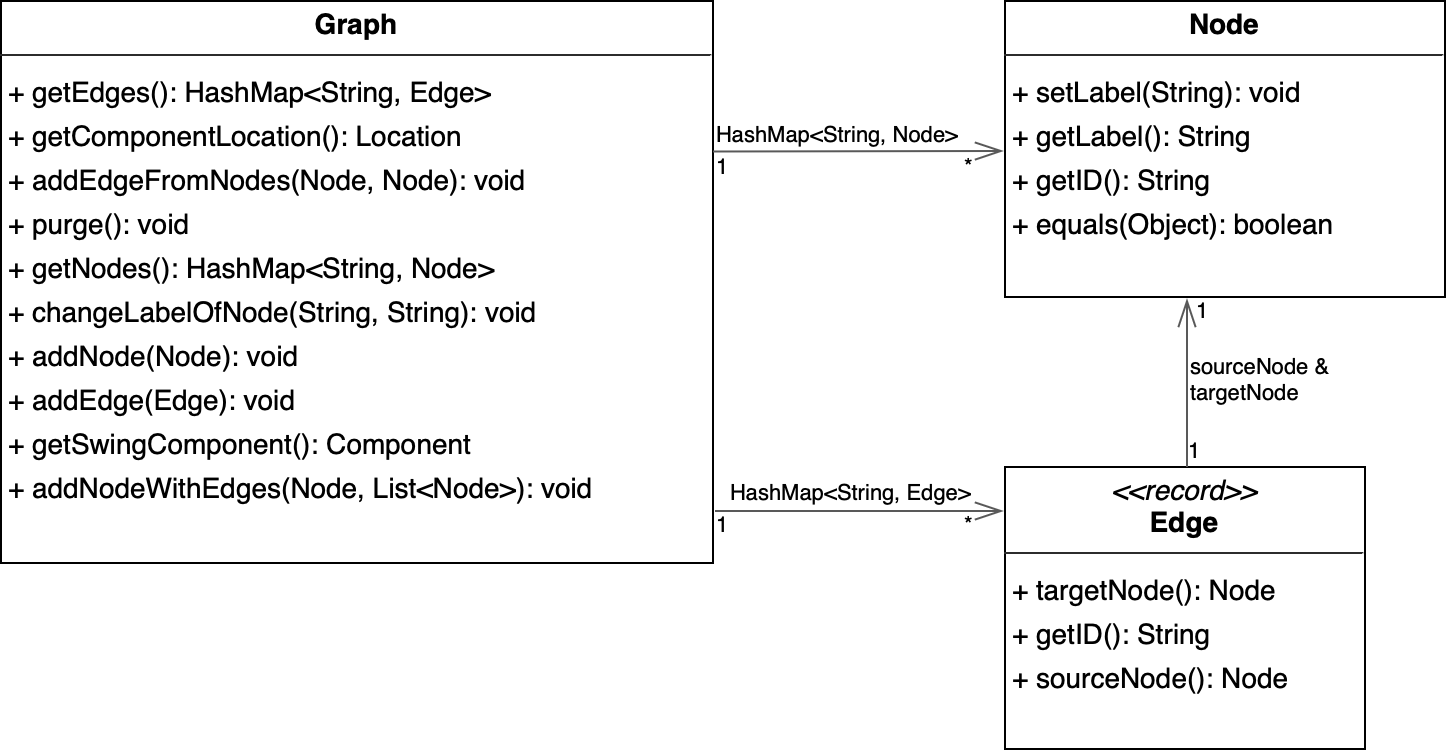
\includegraphics[width=0.99\textwidth]{fig/GUI_Graph_classes_methods.png}
  \caption{Klassenstruktur der Graph-Klassen}%
  \label{fig:graph-classes}
\end{figure}


Hierbei sind die Klassen \textit{Node} und \textit{Edge} Helferklassen, um
anstelle von Strings mit Node- beziehungsweise Edge-Objekten zu arbeiten.\\
Einem \textit{Node}-Objekt wird zu ihrer Erstellung eine eindeutige ID zugewiesen
um das Objekt später mit in einem \textit{GraphStream}-Graphen verwenden zu können.\\
Ein \textit{Edge}-Objekt ist ein Record welcher zwei Node-Objekte
sourceNode und targetNode beinhält. Die für \textit{GraphStream}
eindeutige ID bestimmt sich dann durch die \textit{getID()}-Methode(\cref{cde:edge-id}):

Die \textit{Graph} Klasse ist die zentrale Klasse für die Visualisierung von Graphen.
Sie implementiert das \textit{DataRepresentation} Interface und
alle nötige Kommunikation mit der \textit{GraphStream} Library.

Die im Graph enthaltenen Knoten und Kanten werden in einem \textit{Set} gespeichert(\cref{cde:graph-constructor}),
wenn ein Plugin dem Graphen einen Knoten hinzufügen möchte,
ruft er die Methode \textit{addNode(Node)}(\cref{cde:graph-addNode}) auf.
Diese fügt den Knoten dem Set der im Graphen enthaltenen Knoten hinzu und
fügt den Graphen einen neuen Knoten mit der ID des übergebenen Knotens hinzu.
Anschließend wird die Methode \textit{layout.shake()} aufgerufen.
diese Methode sorgt dafür dass die Anordnung der Knoten neu berechnet wird,
sodass diese immer einen angemessenen Abstand zu einander haben und sich nicht überlappen. 
Analog gibt es auch die Methode \textit{addEdge(Edge)} um Kanten hinzuzufügen
und die Methoden \textit{removeEdge(Edge)} und \textit{removeNode(Node)}
um diese wieder zu entfernen.\\
Um den Graphen komplett zu leeren wurde die Methode \textit{purge()} hinzugefügt.
diese entfernt alle Knoten und Kanten vom Graphen.\\
Um einem Knoten ein Label zu geben, wurde die Methode\\
\textit{setLabelOfNode(Node, String)}(\cref{cde:graph-labelNode})hinzugefügt.

\subsubsection{Tabellen}
\begin{wrapfigure}[15]{r}{0.4\textwidth}
  \centering
  \vspace{-20pt}
  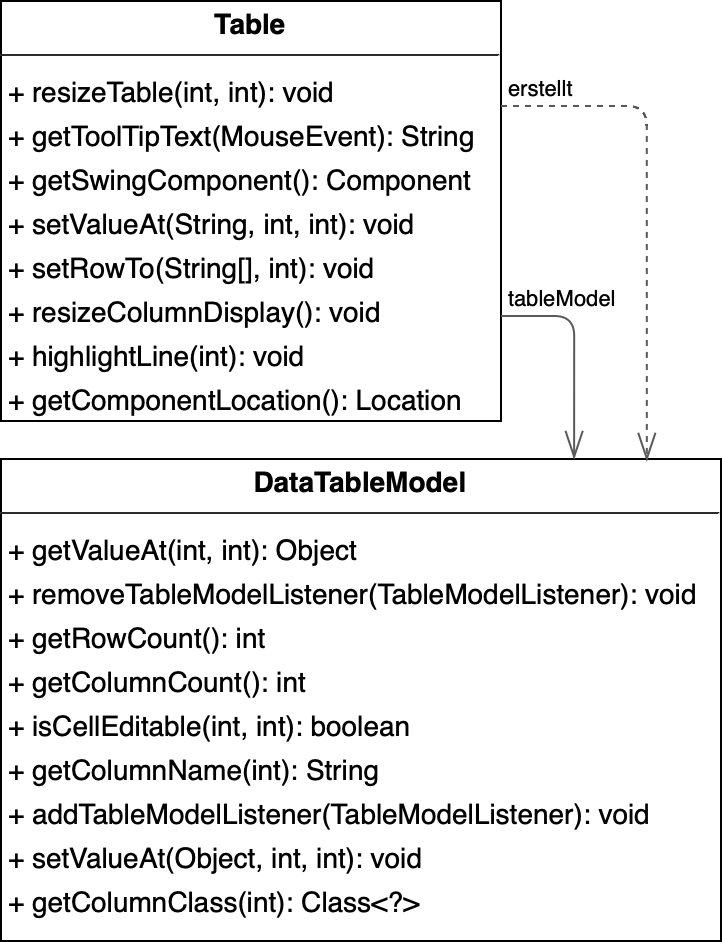
\includegraphics[width=0.33\textwidth]{fig/GUI_Table_classes.png}
  \caption{Klassenstruktur der Tabellenvisualisierung}
  \label{fig:table-classes}
  \vspace{-20pt}
\end{wrapfigure}

Tabellen werden durch die Klasse \textit{Table}(\cref{fig:table-classes}) visualisiert. Da bereits
mit der \textit{JTable} von der \textit{swing}-Library eine
Tabellenvisualisierung angeboten wird, wurde diese auch implementiert.\\
Ein \textit{JTable}-Objekt benötigt immer ein \textit{TableModel}, welches
die Daten, welche dargestellt werden sollen, enthält.\\
Dieses wird von der Klasse \textit{DataTableModel}(\cref{fig:table-classes}) implementiert.
Sie speichert die Daten in einem zweidimensionalen String-Array und implementiert
alle vom \textit{TableModel}-Interface vorgegebenen Methoden.

Die notwendigen, nicht trivialen, Methoden wurden wie folgt implementiert:
\begin{itemize}
  \item \textit{isCellEditable(int, int)} gibt immer \textit{false} zurück,
    da es nicht erwünscht ist, dass der Benutzer die Tabelle bearbeiten kann.
    Ein Plugin kann die Tabelle trotzdem bearbeiten.
  \item Die Methode \textit{getColumnName(int)} gibt immer \textit{null} zurück,
    da in aktuellen Stand des Frameworks Überschriften selber gesetzt werden.
  \item Die Methoden \textit{addTableModeListener(TableModelListener)} und
    \textit{removeTableModeListener(TableModelListener)} fügen eine Implementation
    der Klasse TableModelListener einer zugehörigen Liste hinzu, beziehungsweise
    entfernen sie.
    \footnote{Diese Funktionalität ist notwendig, da das \textit{JTable}-Objekt sich als Listener hinzufügt.} 
  \item \textit{setValueAt(Object, int, int)} versucht den Wert am übergebenen Index
    zu überschreiben. Wenn dies möglich ist werden alle
    Objekte in der TableModelListener Liste benachrichtigt (\cref{cde:setValueAt}).
\end{itemize}


Ein Objekt der \textit{Table}-Klasse (\cref{fig:table-classes}) erweitert die
von \textit{swing} gegebene \textit{JFrame}-Klasse und gibt sich selber in 
\textit{getSwingComponent()} zurück.

Die für Plugins verfügbar gestellten Methoden sind:
\begin{itemize}
  \item Die Methode \textit{resizeTable(int, int)} (\cref{cde:resizeTable}) erstellt ein neues
    \textit{DataTableModel}-Objekt mit der spezifizierten Größe und setzt dieses
    als neues \textit{TableModel}.
  \item \textit{setValueAt(String, int, int)} setzt den übergebenen String
    als Wert an der übergebenen Position indem es \textit{setValueAt(Object, int, int)}
    im \textit{DataTableModel} aufruft.
  \item \textit{setRowTo(String[], int)}
    Setzt die Werte für eine gesamte Zeile indem es über das String-Array iteriert.
  \item \textit{highlightLine(int)} (\cref{cde:highlightLine})
    Markiert die übergebene Zeile.
\end{itemize}

Desweiteren wurden zwei weitere Funktionen implementiert, um Zelleninhalte
besser zu visualisieren:\\
\begin{itemize}
  \item Die Methode \textit{getToolTipText(MouseEvent)} (siehe \cref{cde:tooltip}) überschreibt die in \textit{JTable}
    definierte Methode. Sie erwirkt, dass wenn der Benutzer seine Maus auf eine
    Zelle bewegt, der Inhalt dieser Zelle als ToolTip angezeigt wird. Dies ist gerade dann
    sinnvoll, wenn die Zelle zu klein für ihren Inhalt ist.\\
  \item Die Methode \textit{resizeColumnDisplay()} (siehe \cref{cde:resize}) versucht jeder Spalte die
    kleinstmögliche Breite zu geben und den übrigen Platz auf die letzte Spalte aufzuteilen.
    Dies ist wenn wir 3-Address-Code darstellen wollen sehr sinnvoll, da in der letzten Spalte der Kommentar steht.
\end{itemize}



\newpage
\subsection{Drei Address Code}
Im folgenden Kapitel wird die Implementierung des drei Address Codes erläutert.
Wie zu Beginn von \cref{tac} angeführt werden diese Klassen benötigt:
\begin{figure}[h]
  \centering
  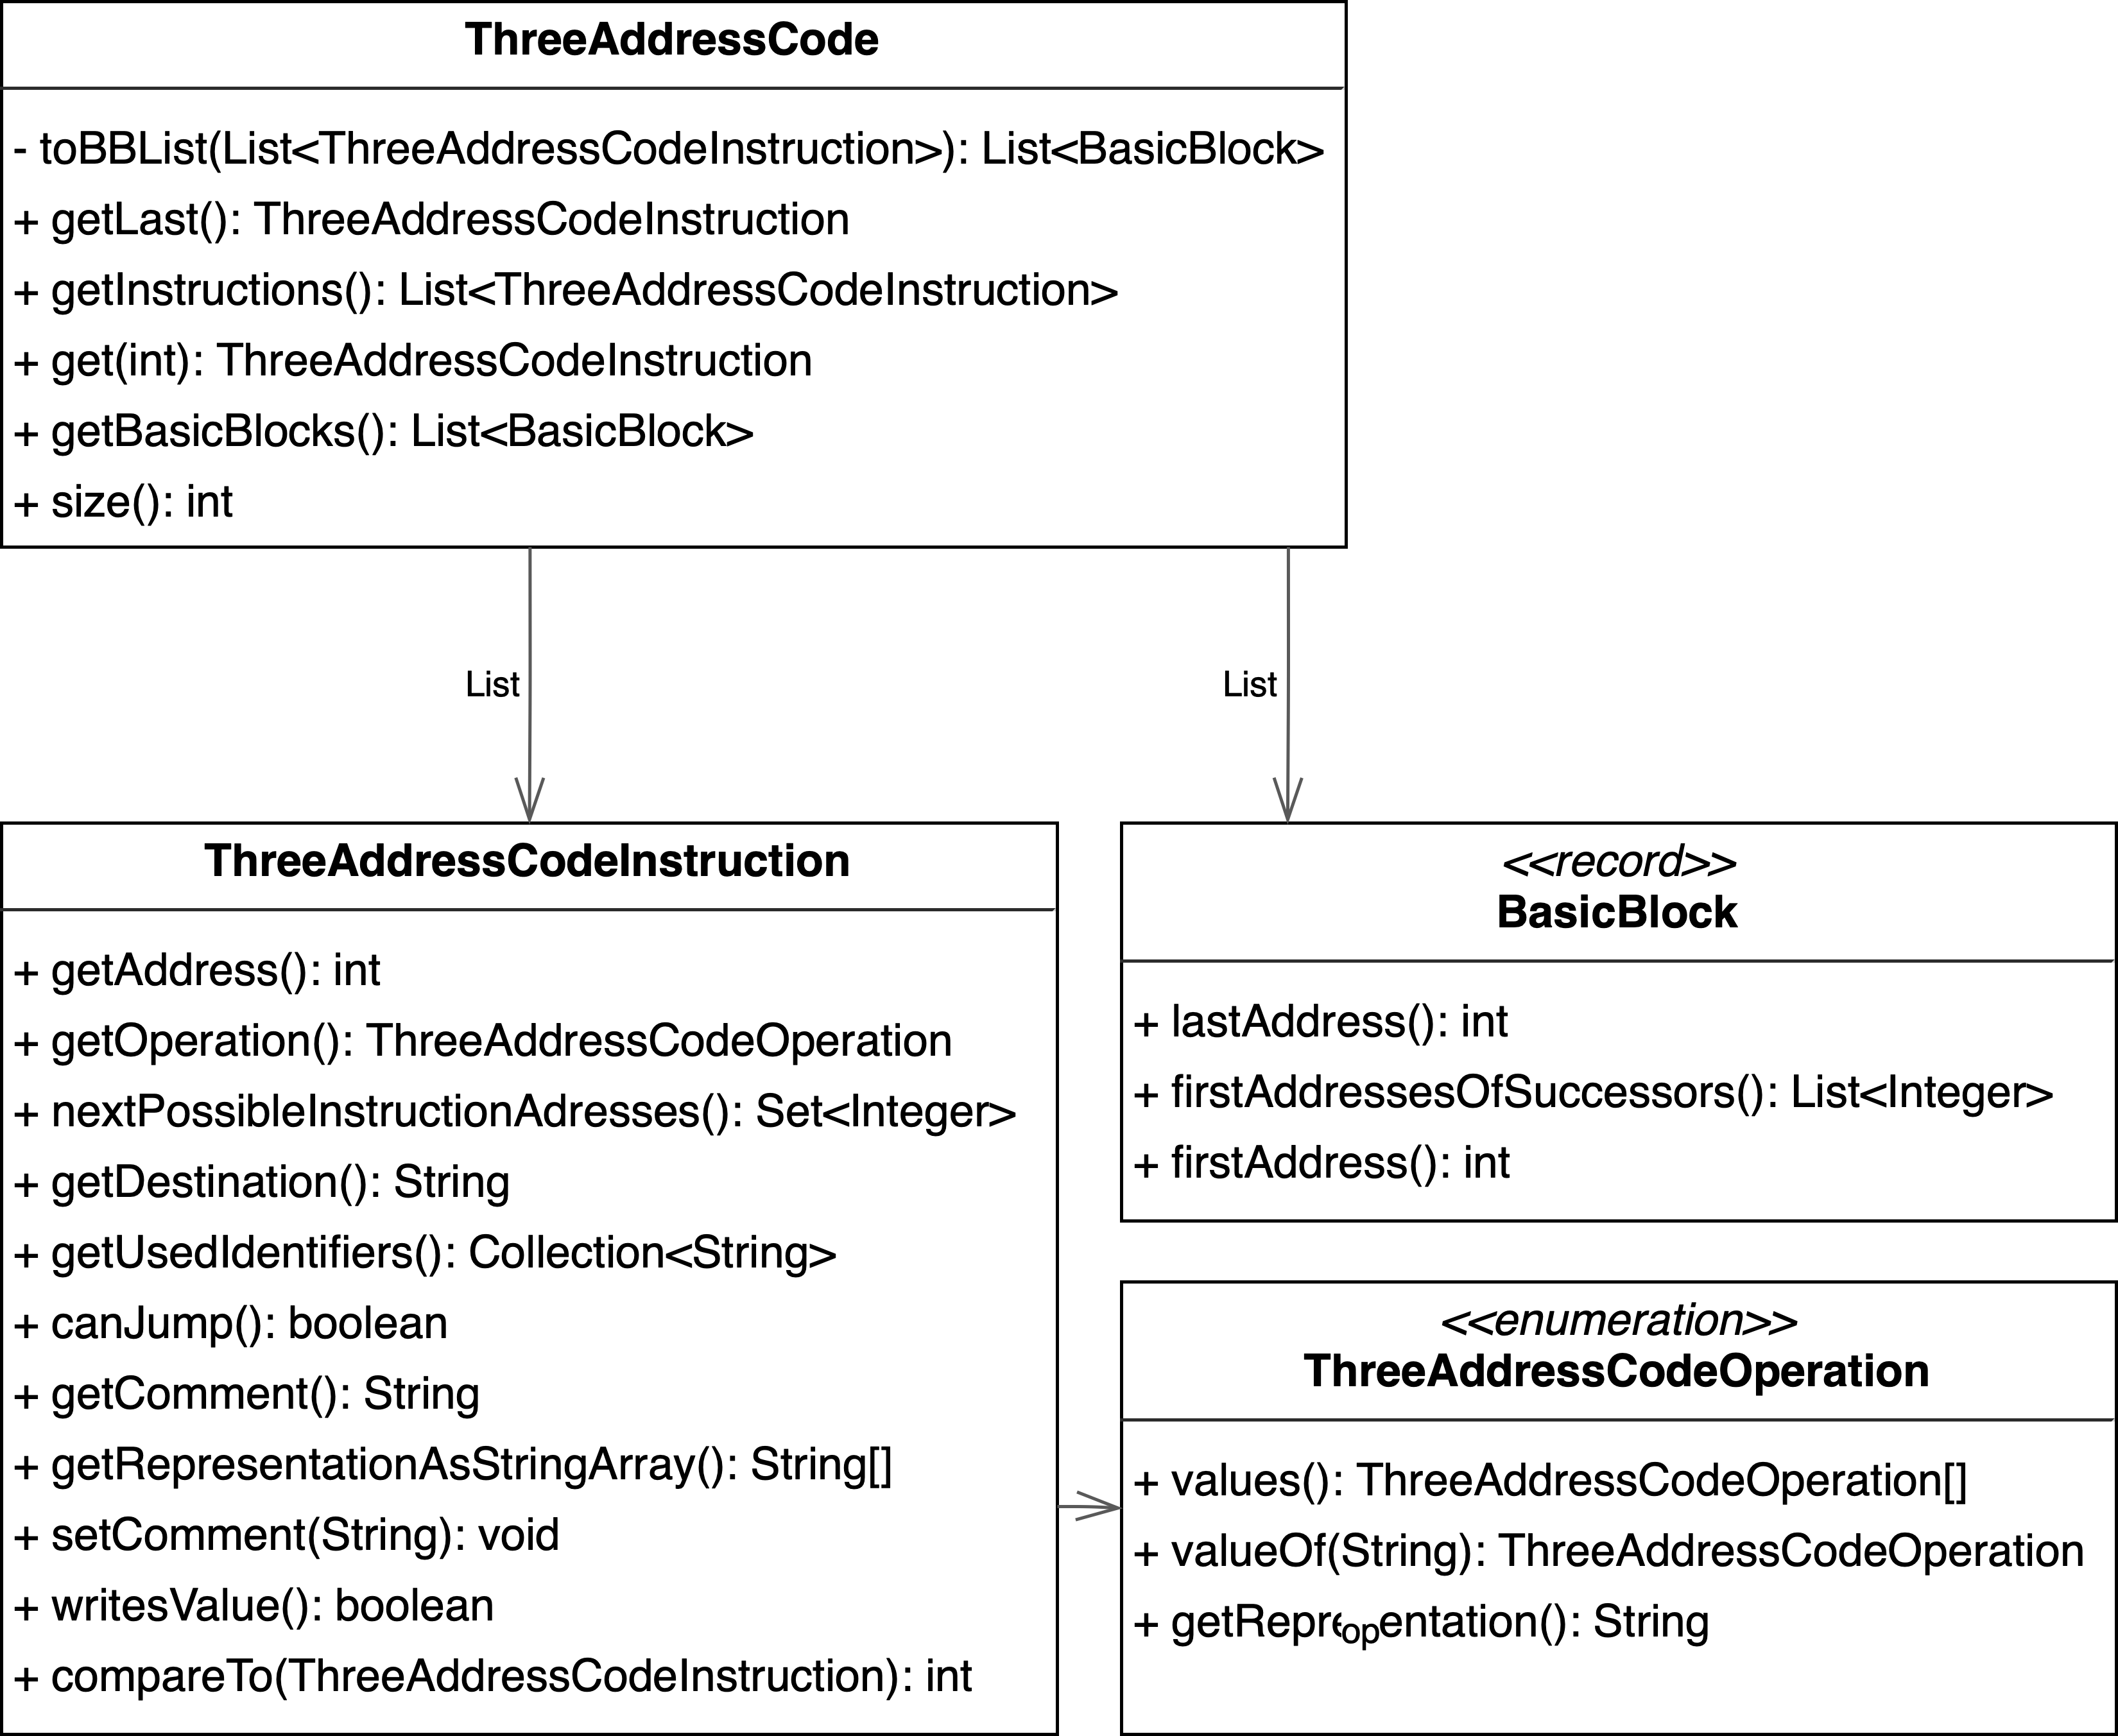
\includegraphics[width=0.98\textwidth]{fig/3AC_classes_methods.png}
  \caption{Implementation der drei Address Code Klassen}
  \label{fig:3ac-classes}
\end{figure}


\newpage
\subsubsection{Die ThreeAddressCodeInstruction Klasse}
\begin{wrapfigure}{r}{0.33\textwidth}
  \centering
  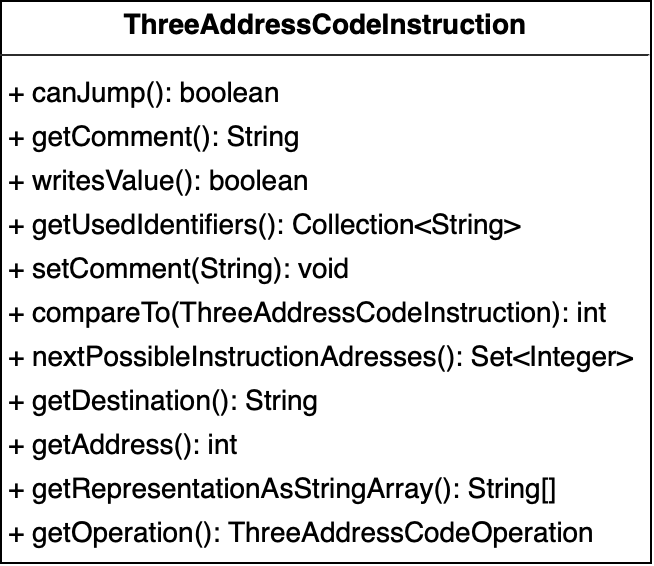
\includegraphics[width=0.4\textwidth]{fig/3AC_ThreeAddressCodeInstruction_methods.png}
  \caption{Die ThreeAddressCodeInstruction Klasse}
  \label{fig:ThreeAddressCodeInstruction}
\end{wrapfigure}

Um einzelne Instruktionen zu modellieren wird die Klasse 
\textit{ThreeAddressCodeInstruction} verwendet.
Generiert werden diese aus einem String und einer Zahl, nämlich der
Addresse an der Stelle ihres Programms.
Dies ist zwar streng gesehen eine Ungenauigkeit der Modellierung, 
da jede Instruktion zwar eine Addresse hat, 
diese jedoch nicht in Bezug direkt auf die einzelne Instruktion steht,
sondern nur im Kontext des Gesamtprogrammes gesehen werden kann.\\
Da es jedoch die Implementierung einiger folgender Methoden stark vereinfacht
und keine Instruktion ohne eindeutige Addresse an der sie gespeichert oder ausgeführt werden kann
existiert wurde sich dazu entschieden für diese ein Attribut anzulegen.\\

Um die in \cref{t:tac} definierten Instruktionen zu modellieren werden folgende
weitere Attribute benötigt:
\begin{enumerate}
  \item Eine \textit{ThreeAddressCodeOperation}. Dies ist ein Enum, welches definiert
    welche Operation die angegebene Instruktion ausführt.
  \item Ein String namens \textit{destination}. Dieser gibt entweder das Ziel eines Sprunges an,
    oder den Ort an dem eine Berechnung gespeichert werden soll.
  \item Den String \textit{source}. Da alle Instruktionen ausser dem unbedingten Sprung
    mindestens einen Wert verarbeiten.
  \item Und einen String \textit{modifier}, für Instruktionen die zwei Werte
    entweder vergleichen oder arithmetisch verrechnen.
\end{enumerate}
Desweiteren wurde ein weiteres String-Attribut \textit{comment} zum speichern von Kommentaren
hinzugefügt.

Um aus dem Eingabestring ein passendes \textit{ThreeAddressCodeInstruction}-Objekt
zu generieren wird der Eingabestring im Konstruktor(\cref{cde:taci-constructor})
in seine Bestandteile aufgelöst und der richtigen Instruktion zugeordnet.

\newpage
Außerdem wurden folgende Helfermethoden, welche im späteren Verlauf dieser Arbeit
benötigt werden, implementiert:
\begin{enumerate}
  \item Die Methode \textit{canJump()} gibt den Wahrheitswert \textit{wahr} zurück, wenn die
    Instruktion springen kann oder immer springt, ansonsten gibt sie \textit{falsch} zurück.
  \item Die Methode \textit{writesValue()} gibt den Wahrheitswert \textit{wahr} zurück,
    wenn die Instruktion den Wert der in \textit{destination} gespeichert ist überschreibt.
    Ansonsten gibt sie \textit{falsch} zurück.
  \item \textit{getUsedIdentifiers()} gibt die Menge der Werte in \textit{source} und \textit{modifier} zurück,
    wenn diese Variablen referenzieren und keine Konstanten sind.
  \item Die Methode \textit{compareTo(ThreeAddressCodeInstruction)} implementiert das Interface
    Comparable<>. Wir sehen später dass dies sinnvoll ist wenn in Erfahrung gebracht werden
    soll sich ob zwei Instruktionen im selben Grundblock befinden.
  \item \textit{nextPossibleInstructionAddresses()} gibt die Menge der nächsten möglichen 
    Instruktionsaddressen zurück. Dies ist in den meißten Fällen einfach die nächste
    Addresse, wenn die aktuelle Instruktion jedoch ein unbedingter Sprung ist, ist es der
    Wert in \textit{destination}, wenn die Instruktion ein bedingter Sprung ist, wird sowohl die
    nächste Addresse als auch der Wert in \textit{destination} zurückgegeben.
  \item Die Methode \textit{getRepresentationAsStringArray()} gibt
    eine Repräsenationen der Instruktion als \textit{String[]} in der Form zurück, 
    dass sie nacheinander die eingelesene Instruktion bilden zum Beispiel:
\end{enumerate}
Die restlichen in \textit{ThreeAddressCodeInstruction} enthaltenen Klassen sind getter und setter Methoden.

\subsubsection{Die BasicBlock Record-Klasse}
\begin{wrapfigure}{r}{0.35\textwidth}
  \vspace{-15pt}
  \centering
  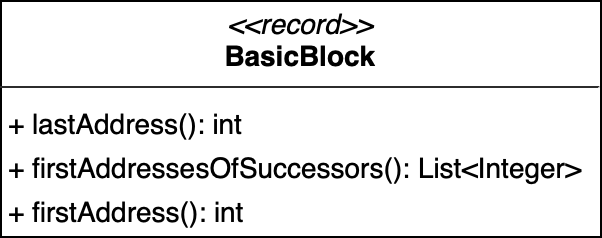
\includegraphics[width=0.35\textwidth]{fig/3AC_BasicBlock_methods.png}
  \caption{Die ThreeAddressCodeInstruction Klasse}
  \label{fig:BasicBlock}
\end{wrapfigure}
Um die Grundblöcke eines Programmes zu modellieren reicht uns eine Record-Klasse,
da Grundblöcke immer ein gesamtes Programm partitionieren reicht es die erste und 
letzte der enthaltenen und die Menge der folgenden Addressen zu kennen.\\


\newpage
\subsubsection{Die ThreeAddressCode Klasse}
\begin{wrapfigure}{r}{0.4\textwidth}
  \vspace{-15pt}
  \centering
  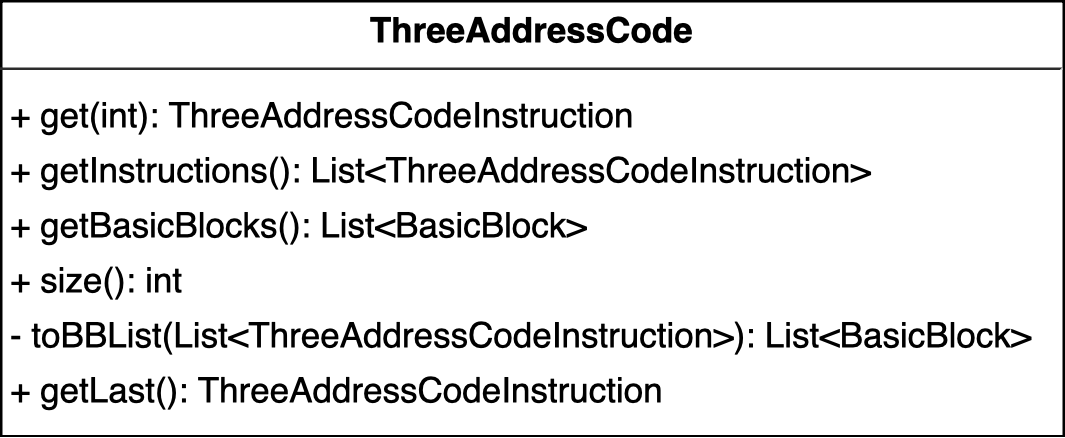
\includegraphics[width=0.4\textwidth]{fig/3AC_class_methods.png}
  \caption{Die ThreeAddressCode Klasse}
  \label{fig:ThreeAddressCode}
\end{wrapfigure}

Die Klasse \textit{ThreeAddressCode} agiert im Framework als Modellierung eines
gesamten Programmes. Sein Konstruktor(\cref{cde:tac-constructor}) wird mit
einem String aus 3-Address-Code Instruktionen welche durch einen Zeilenumbruch getrennt sind
aufgerufen, daraus generiert er eine Liste and \textit{ThreeAddressCodeInstruction}
Objekten und aus diesen Objekten wiederum eine Liste an \textit{BasicBlock} Objekten.

Die Methode \textit{toBBList(List<ThreeAddressCodeInstruction>)} ist hier eine statische Methode, welche für eine
Liste an \textit{ThreeAddressCodeInstruction}-Objekten eine Liste an \textit{BasicBlock}-Objekten
zurückgibt. Dafür wurde der in \cref{t:bb} angegebene Algorithmus implementiert(\cref{cde:bb-gen}).
In Folge dessen werden die nächstmöglichen Instruktionsaddressen bestimmt.

Um alle Leader zu finden wurde wie folgt über die Instruktionsliste iteriert(\cref{cde:bb-leader}).
Wenn die Instruktion an der Stelle i springen kann, ist das Ziel des Sprungs ein Leader.\\
Ausserdem ist die Instruktion an der Stelle i+1 auch ein Leader, wenn sie existiert
Um die ersten Addressen der Nachfolger zu erhalten, schauen wir uns die letzte
Addresse unseres Blockes an(\cref{cde:bb-successor}), da an dieser entweder entweder ein Sprung ist,
an die nächste Addresse gesprungen wird oder das Programm zu ende ist.
Mit diesen Klassen und Methoden wurden alle für die Implementation der Plugins
notwendigen Modellierungen abgebildet. 


\newpage
\subsection{Implementierung von Algorithmen}
\begin{wrapfigure}[18]{r}{0.475\textwidth}
  \centering
  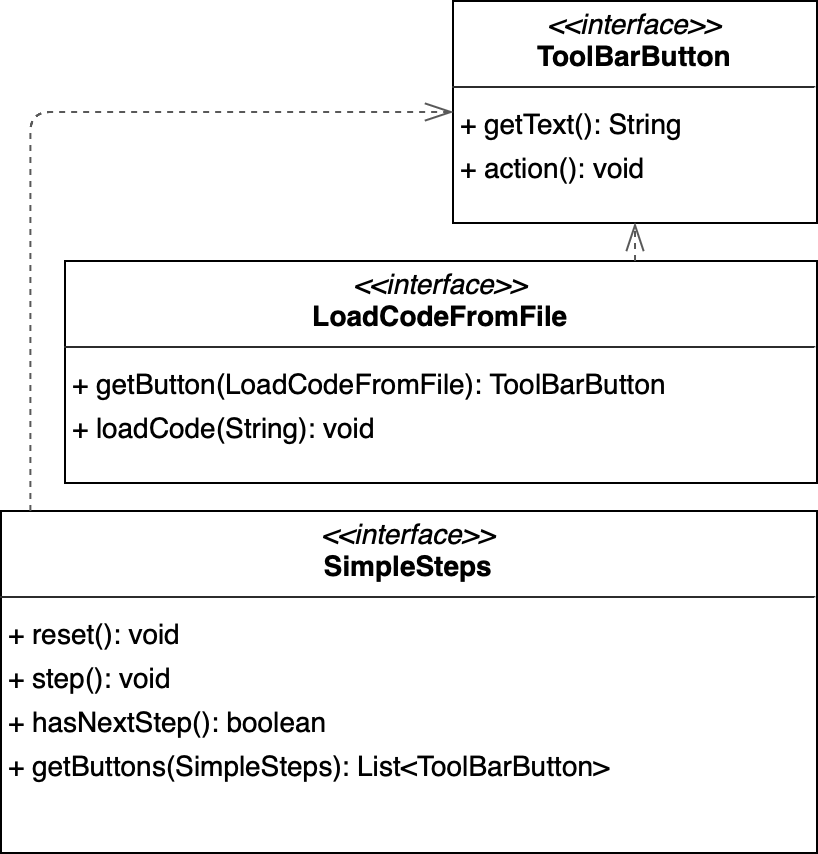
\includegraphics[width=0.47\textwidth]{fig/GUI_ToolBar_classes_methods.png}
  \caption{Das ToolBarButton Interface}
  \label{fig:ToolBarButtons}
\end{wrapfigure}


Dieser Abschnitt befasst sich damit wie Algorithmen als Plugins implementiert werden,
sodass diese vom Framweork richtig visualisiert werden.

Hierbei gibt es zwei Interfaces die Implementiert wurden, das \textit{Plugin} Interface
und das \textit{ToolBarButton} Interface.
Letzteres spezifiziert alle Buttons welche in der Toolbar angezeigt werden
wenn das Plugin geladen ist. Es ist sehr einfach aufgebaut und verfügt nur über zwei Methoden.
Eine Methode \textit{getText()} gibt einen String zurück, welcher im Button angezeigt wird.
Die andere Methode \textit{action()} wird ausgeführt wenn der Nutzer auf den zugehörigen Button drückt.\\
Da alle in dieser Arbeit implementierten Algorithmen sowohl Schrittweise durchlaufen werden
sollen als auch Code laden müssen wurden ausserdem zwei Interfaces implementiert
welche ToolBarButtons für Plugins bereitstellen.

Das Interface \textit{LoadCodeFromFile} stellt sicher dass es eine Funktion \textit{loadCode(String)}
gibt, in die Code als ein String in das Plugin geladen werden kann.\\
Die Funktion \textit{getButton()} ist hier eine statische Funktion, welche eine Implementation
von \textit{ToolBarButton} zurückgibt welche zuerst einen \textit{JFileChooser}
\footnote{\textit{JFileChooser} ist eine Klasse aus der \textit{swing}-Library welche eine Bedienfläche zum öffnen von Dateien bietet}
öffnet und dann die Datei als String lädt. Hierbei wird auch der Unterschied
zwischen Windows und *nix basierenden Systemem berücksichtigt und die einzelnen
Zeilen nur mit einem Zeilenumbruch(\textbackslash n) konkateniert.

Das Interface \textit{SimpleSteps} implementiert sogar drei Buttons und somit auch
drei Methoden. Ein Reset Button, der die Methode \textit{reset()} aufruft, ein Step
Button, der die Methode \textit{step()} aufruft und einen Run Button, der die Methode
\textit{step()} so lange aufruft wie die Methode \textit{hasNextStep() wahr} zurückgibt.
Diese drei Buttons werden wieder in einer statischen Funktion \textit{getButtons()}
generiert.\\


\newpage
\subsubsection{Das Plugin Interface}
\begin{wrapfigure}[4]{r}{0.5\textwidth}
  \centering
  \vspace{-20pt}
  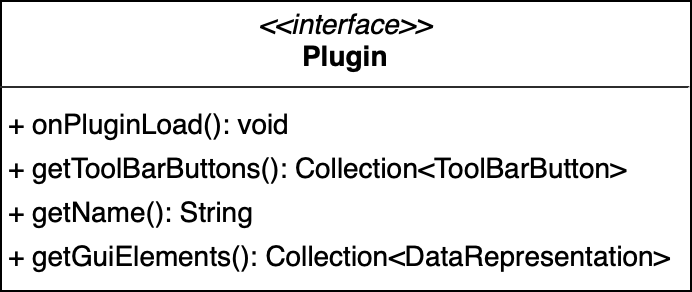
\includegraphics[width=0.46\textwidth]{fig/Plugin_methods.png}
  \caption{Das Plugin Interface}
  \label{fig:PluginInterface}
  \vspace{-20pt}
\end{wrapfigure}

Das \textit{Plugin}-Interface (\cref{fig:PluginInterface}) beschreibt die
Schnittstelle zwischen dem Framework und dem entwickelten Plugin.
Um ein Plugin zu Implementieren benötigt es folgende Methoden:
\vspace{30pt}

\begin{itemize}
  \item \textit{onPluginLoad()} wird ausgeführt wenn das Plugin geladen wird, also zum 
    Beispiel wenn der Nutzer im Plugin Dropdown Menü auf den Button mit dem Namen des
    Plugins drückt.
  \item \textit{getToolBarButtons()} gibt eine Collection der implementierten \textit{ToolBarButtons}
    zurück, sodass diese wenn das Plugin geladen wird in die ToolBar eingefügt werden.
  \item \textit{getName()} gibt den Namen des Plugins zurück, sodass er im Plugin Dropddown Menü
    angezeigt wird.
  \item \textit{getGuiElements()} gibt eine Collection der \textit{DataRepresentation} Elemente
    zurück die das Plugin anzeigen soll.
\end{itemize}
Mehr Abstraktionen braucht das Framework nicht um alle Algorithmen die in dieser
Arbeit implementiert werden sollten zu Visualisieren.
Im nächsten Kapitel wird nun auf die spezifische Implementationen der Algorithmen eingegangen.
